\documentclass[10pt]{beamer}

\usetheme{metropolis}
\usepackage{appendixnumberbeamer}

\usepackage{booktabs}
\usepackage[scale=2]{ccicons}
\usepackage{graphicx}
\usepackage{pgfplots}
\usepgfplotslibrary{dateplot}
\usepackage{caption}
\usepackage{subcaption}
\usepackage{xspace}
\newcommand{\themename}{\textbf{\textsc{metropolis}}\xspace}

\title{Bhabha Tracking Efficiencies}
%\subtitle{A modern beamer theme}
\date{01.03.2019}
\author{Martin Sobotzik}
\institute{Johannes Gutenberg Universit\"at Mainz}
% \titlegraphic{\hfill
\includegraphics[height=1.5cm]{logo.pdf}}

\begin{document}

\maketitle
{%
\setbeamertemplate{frame footer}{Bhabha Tracking Efficiencies}

%\section{Reproducing Plots}


\begin{frame}{Getting Started}

\begin{itemize}	
	\item I want to study the tracking efficiency of Bhabha processes
	\item For this I look at electrons which are only detected by the CDC.
	\item They are therefor labeled and treated as gammas
	
	\item Filling the gamma lists:
	
	\begin{itemize}
		\item gamma:probe '$(\textrm{E} > 0.1 )$'
		\item gamma:tag '$(\textrm{clusterE} > 3.0)$'
		\item vpho:cand 'reconstructed from gamma:probe and gamma:tag'
	\end{itemize}

	\item What cuts do we need to do this? (Sam's email)
		\begin{itemize}
			\item $0.296706 < \theta < 2.61799 \rightarrow$ It has to hit the CDC
			\item $\textrm{nCleanedTracks}[ \textrm{abs}(\textrm{dz}) < 2.0 \textrm{ and } \textrm{abs}(\textrm{dr}) < 0.5 \textrm{ and nCDCHits} > 0 \textrm{ and pt } > 0.15] < 1 \rightarrow $ bad quality hits 
			\item $\textrm{M}(\textrm{vpho}) > 8.0\,\textrm{GeV} \rightarrow $ To Cut away background (not from his email by surely he is using something like that)					
		\end{itemize}
	
\end{itemize}	
\end{frame}

\begin{frame}{Reproducing Plots}
	
	\begin{itemize}
		\item Running on Data Prod6
		\item /hsm/belle2/bdata/Data/release-02-01-00/DB00000438 /prod00000006/e0003/4S/r02*/all/mdst.sub00/*.root
		\item Sam's plots are on the left.	
		\item Three lines. The middle one is $\gamma \gamma$ the two others are $\textrm{ee}$
\end{itemize}
	
	
	\begin{figure}
		\centering
		\begin{subfigure}{.5\textwidth}
			\centering
			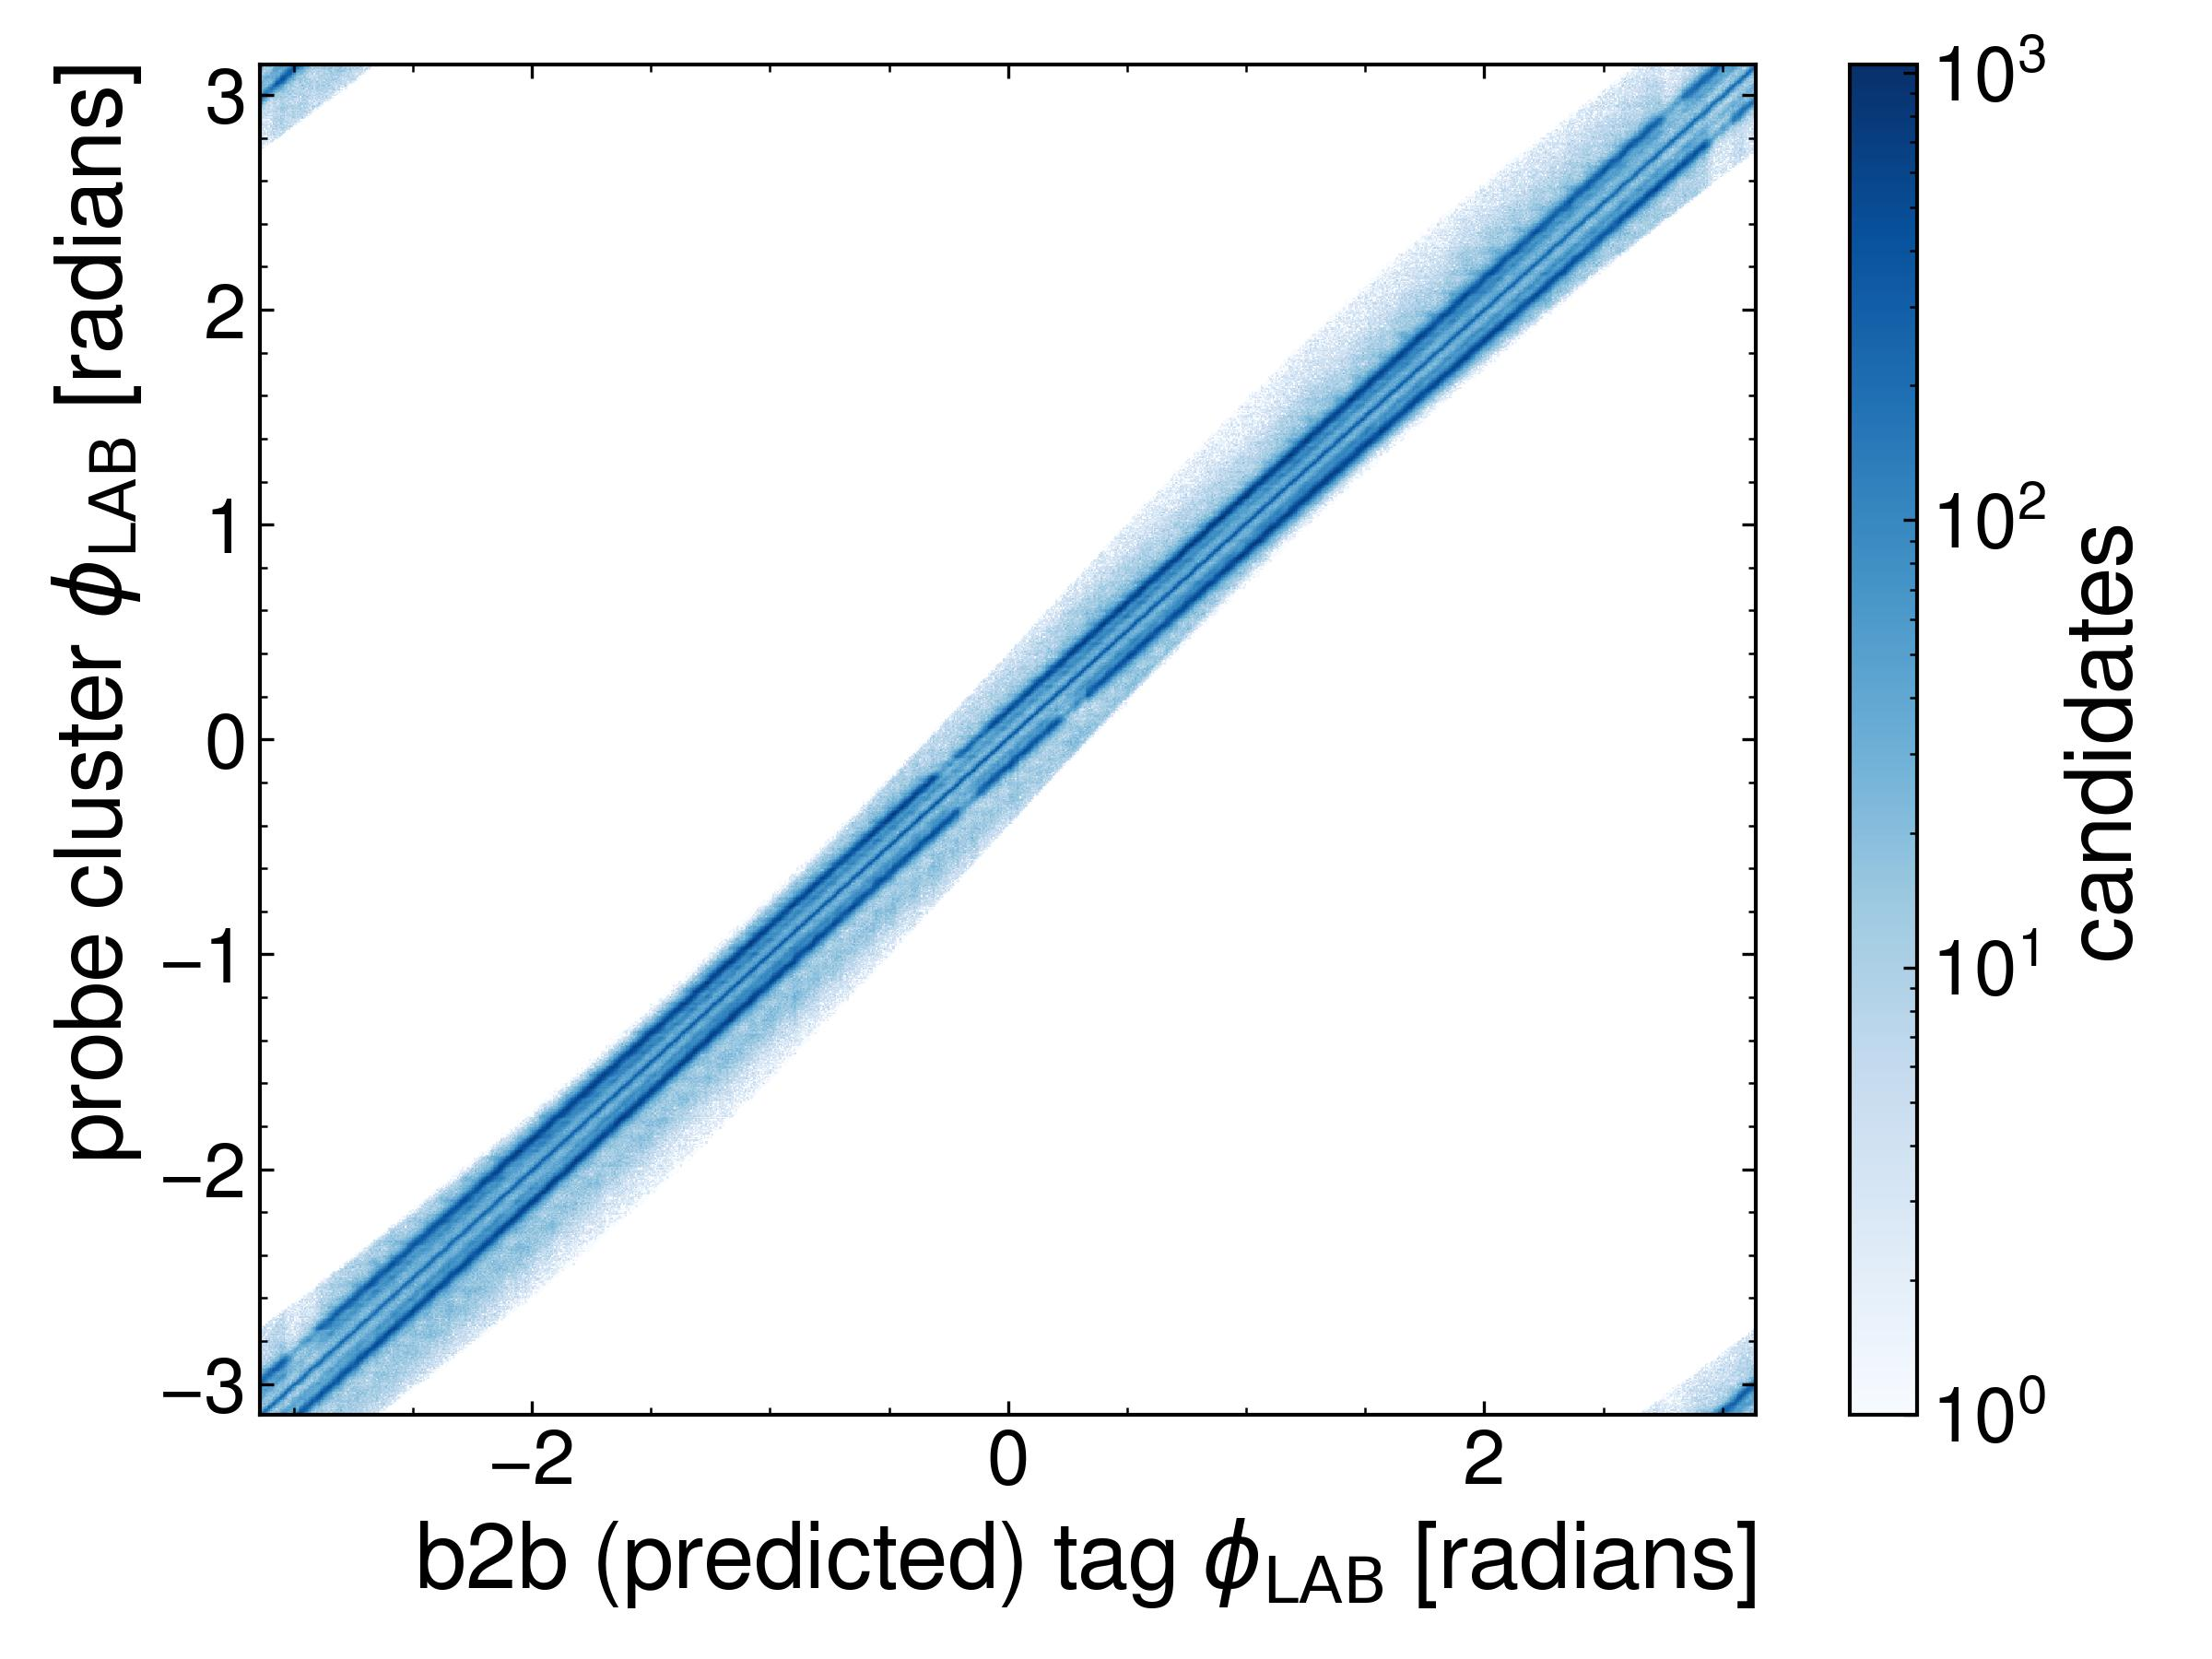
\includegraphics[width=5.4cm]{Plots/prodRecSam.jpeg}
			
			\label{fig:sub1}
		\end{subfigure}%
		\begin{subfigure}{.5\textwidth}
			\centering
			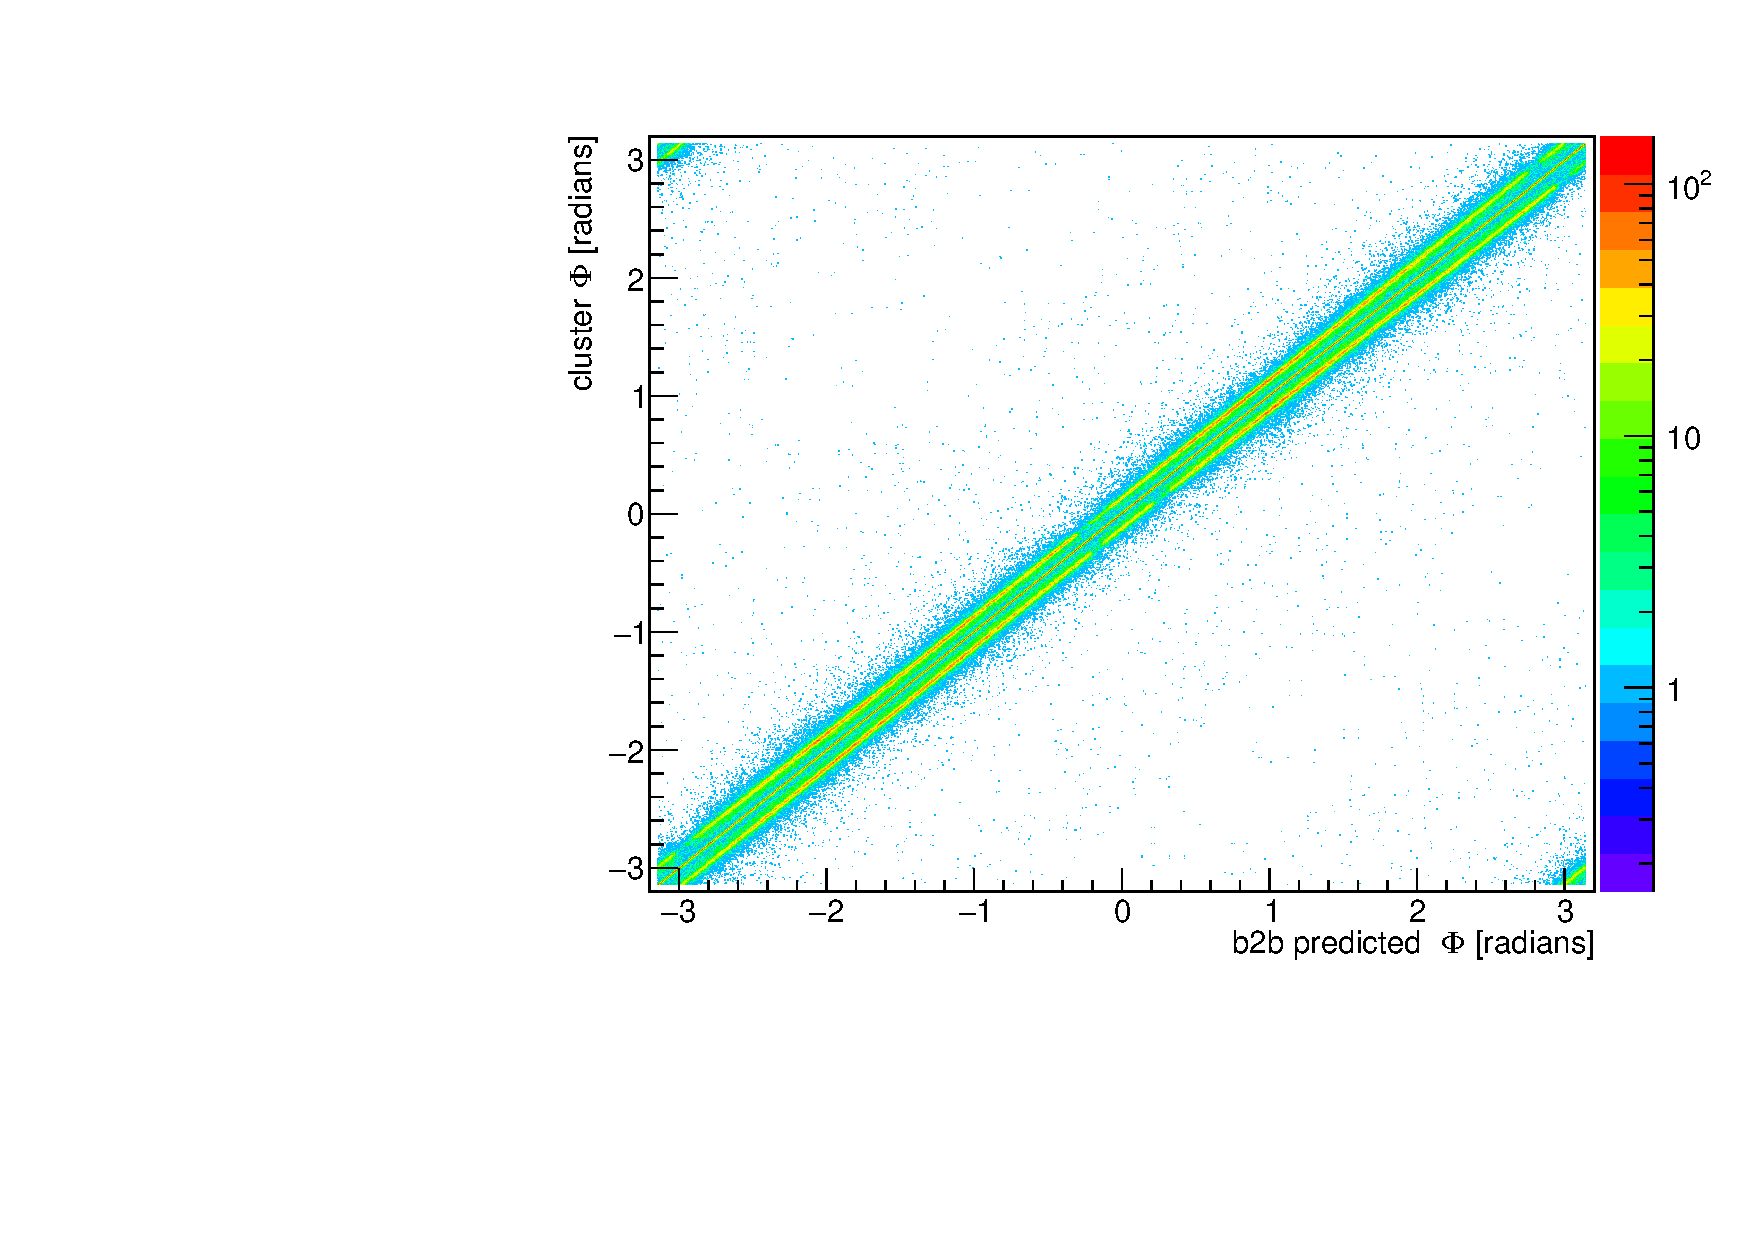
\includegraphics[width=5cm]{Plots/clusterb2b}
			
			\label{fig:sub2}
		\end{subfigure}
				
		\label{fig:test}
	\end{figure}
	
	
\end{frame}


\begin{frame}{Reproducing Plots}
	
	Same plots but zoomed in
	
		\begin{figure}
		\centering
		\begin{subfigure}{.5\textwidth}
			\centering
			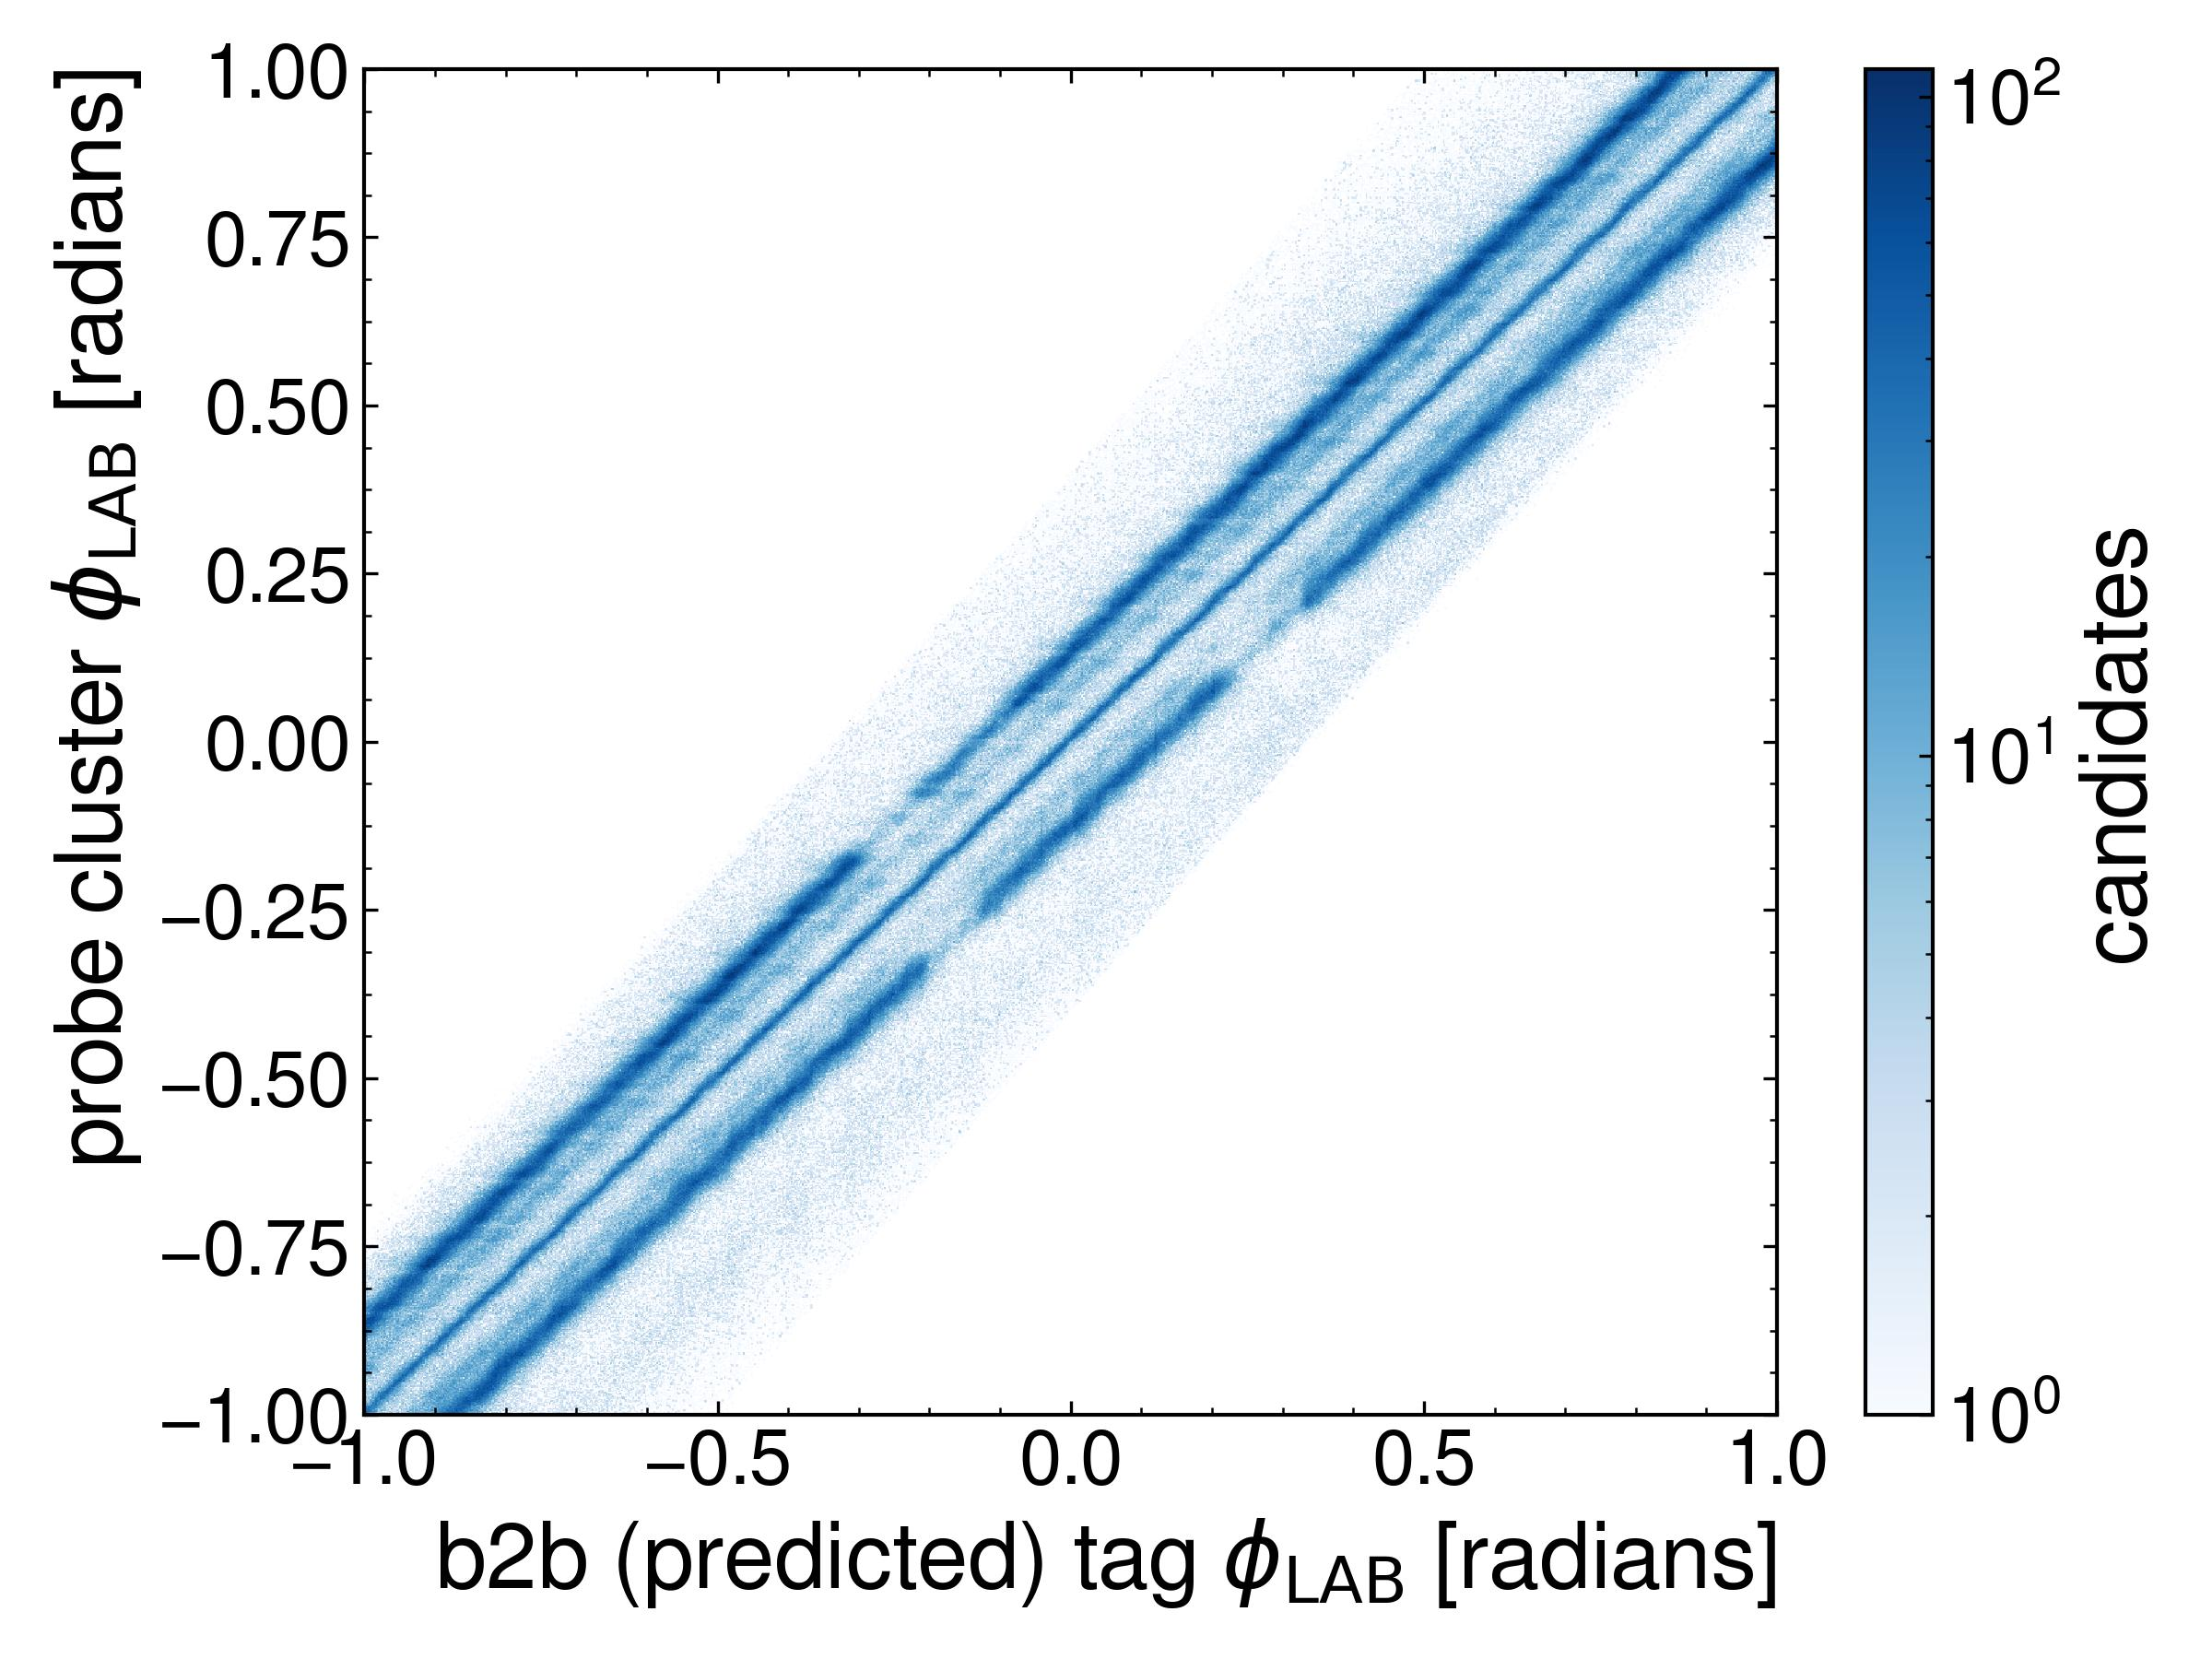
\includegraphics[width=5.4cm]{Plots/ZommedSam.jpeg}
			
			\label{fig:sub1}
		\end{subfigure}%
		\begin{subfigure}{.5\textwidth}
			\centering
			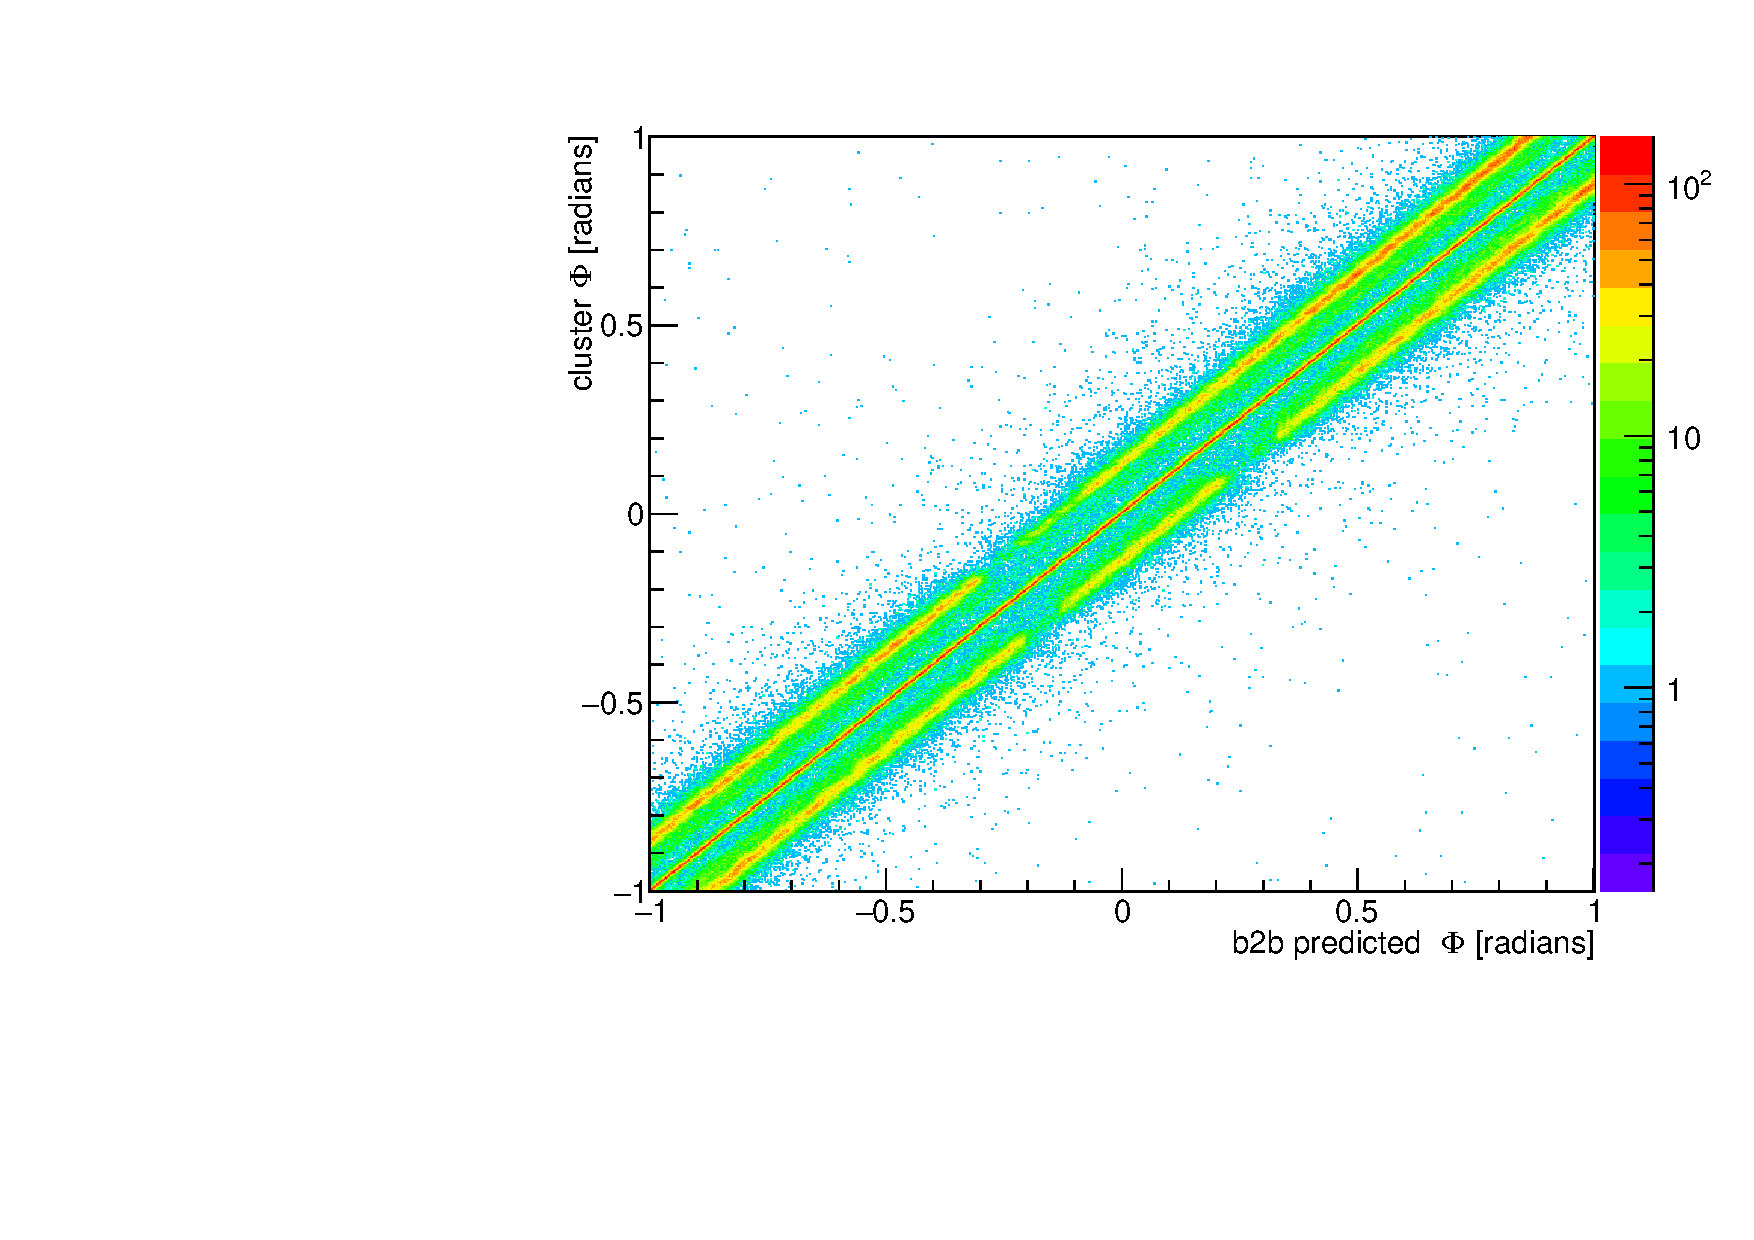
\includegraphics[width=5cm]{Plots/zommedb2b}
			
			\label{fig:sub2}
		\end{subfigure}
		
		\label{fig:test}
	\end{figure}
		
\end{frame}


\begin{frame}{Reproducing Plots}
\begin{itemize} 
	\item The middle peak is $\gamma \gamma$ the two other peaks are $\textrm{ee}$
	\item My $\gamma \gamma$ peak is way higher (Maybe different mass cut?)

\end{itemize}
\begin{figure}
	\centering
	\begin{subfigure}{.5\textwidth}
		\centering
		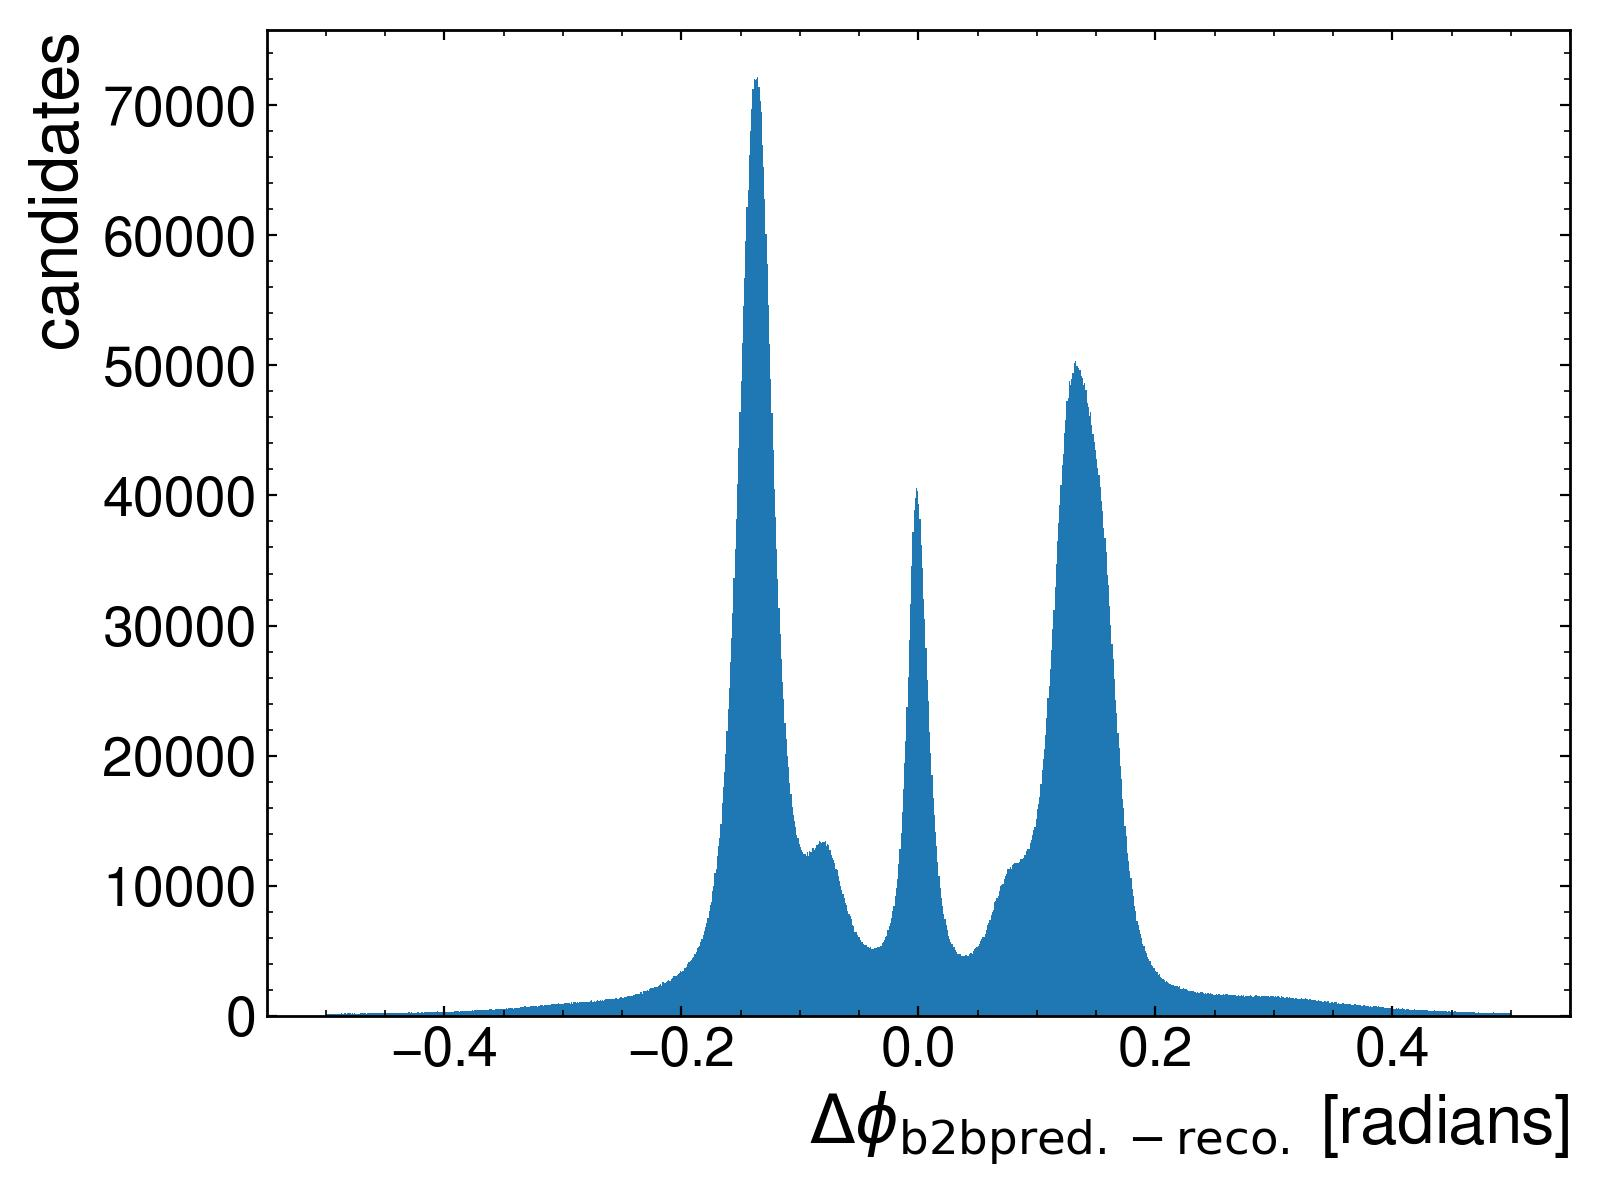
\includegraphics[width=5.4cm]{Plots/deltaPhiSam.jpeg}
	
		\label{fig:sub1}
	\end{subfigure}%
	\begin{subfigure}{.5\textwidth}
		\centering
		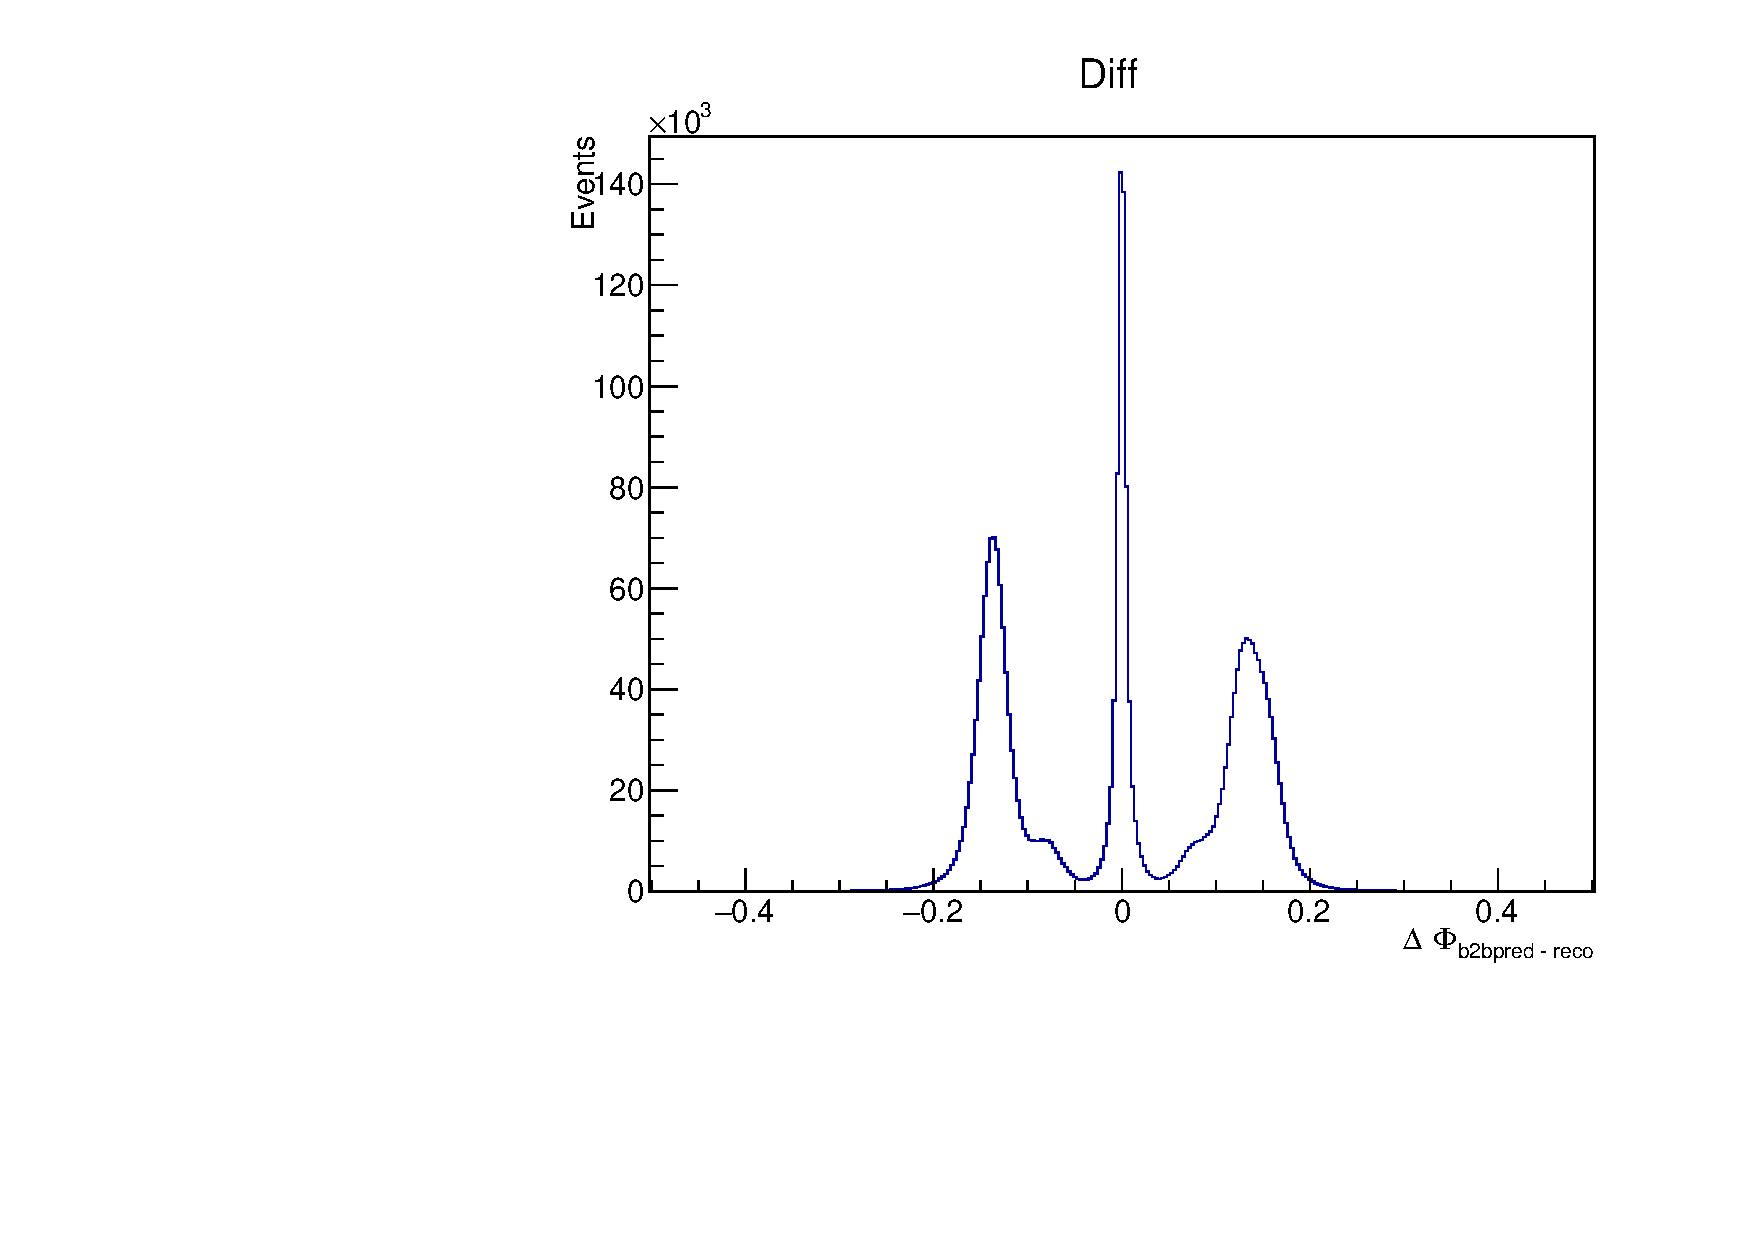
\includegraphics[width=5cm]{Plots/DeltaPhi.pdf}
	
		\label{fig:sub2}
	\end{subfigure}

	\label{fig:test}
\end{figure}

\end{frame}


\begin{frame}{Some more plots}

Here is no Mass cut on the vpho

	
	\begin{figure}
		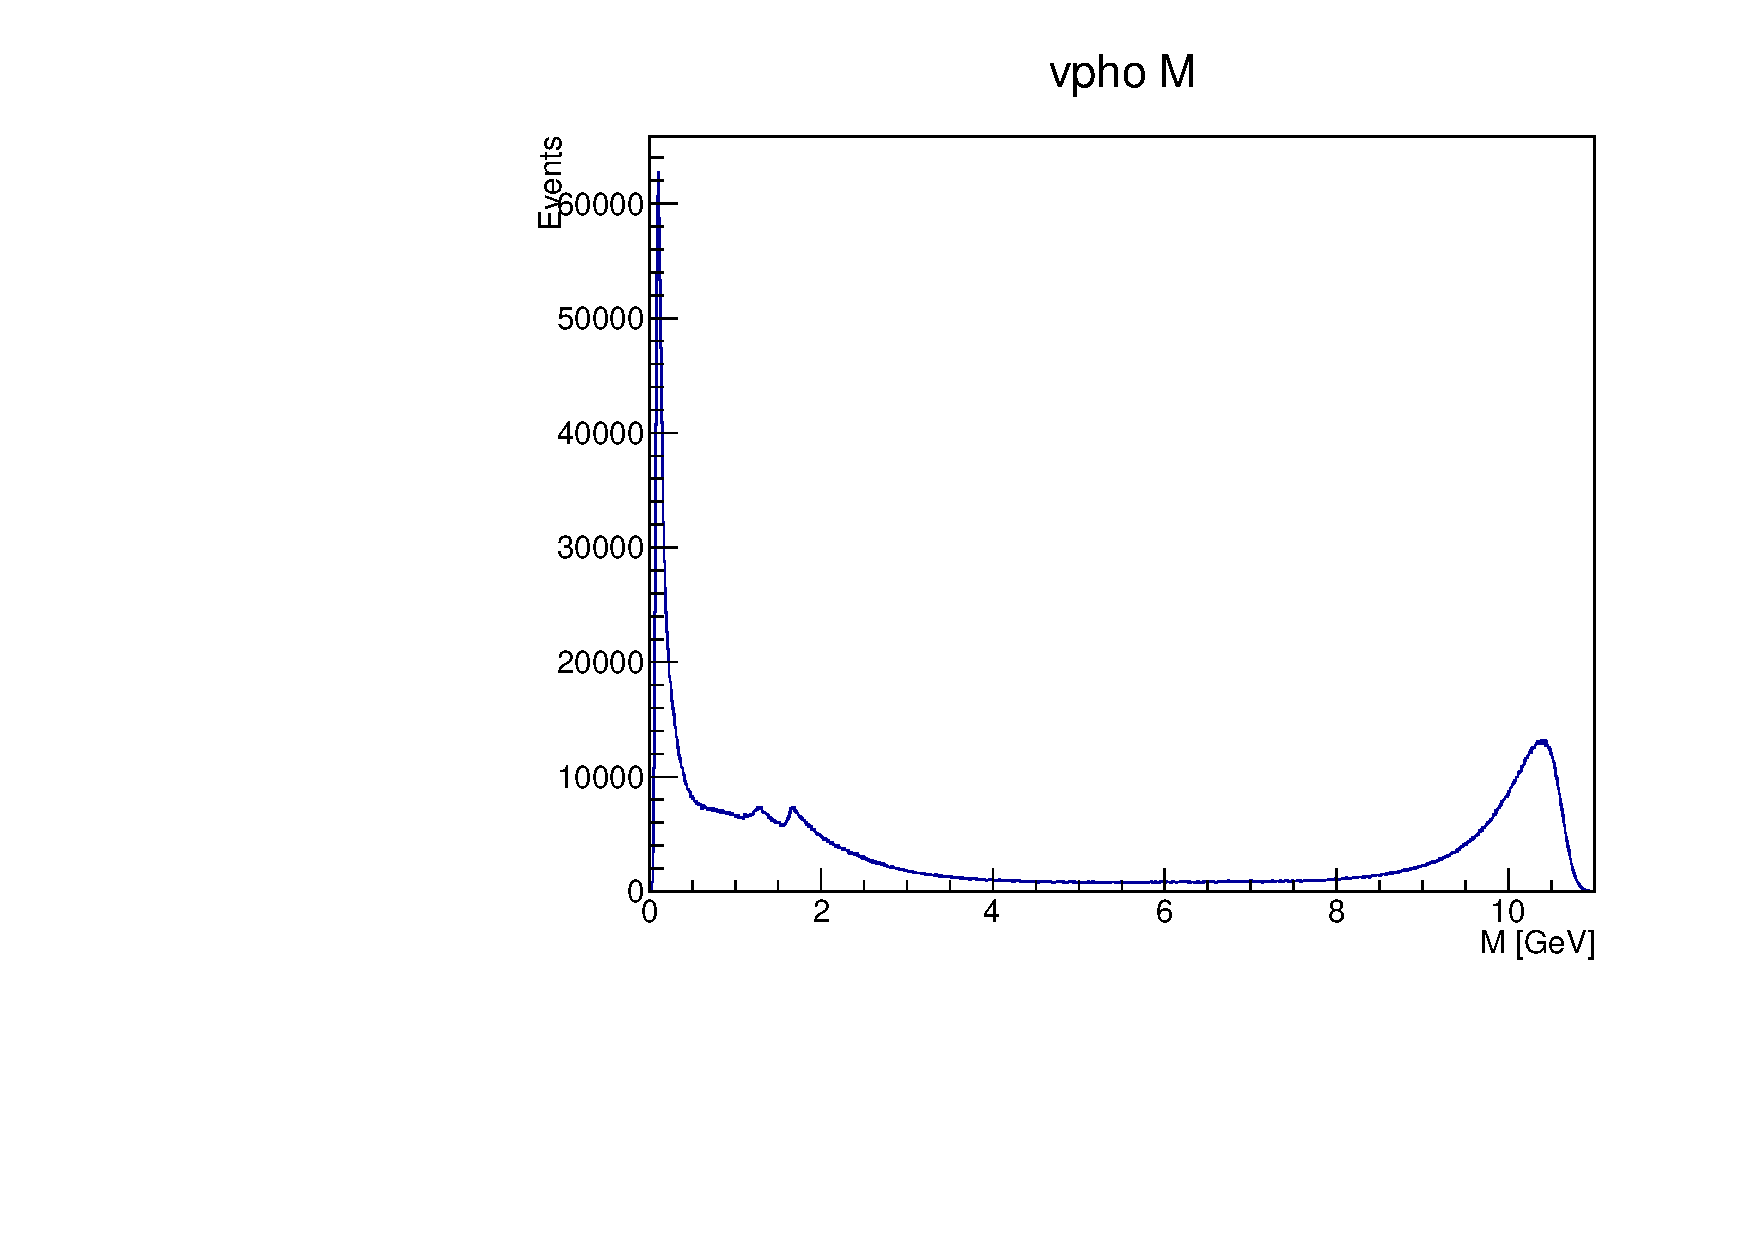
\includegraphics[width=8cm]{Plots/vphoM.pdf}
	\end{figure}
	
	
\end{frame}



\begin{frame}{Some more plots}
	
	\begin{figure}
		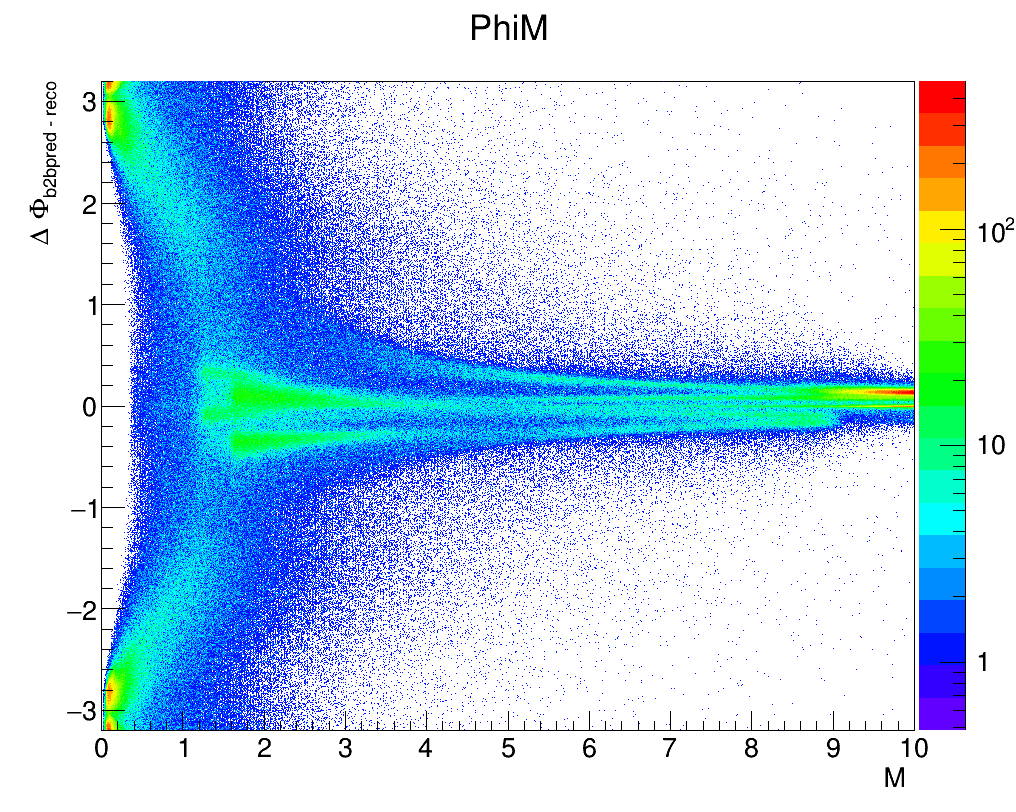
\includegraphics[width=8cm]{Plots/PhiM.png}
	\end{figure}
	
	
\end{frame}

\begin{frame}{Some more plots}
	
	\begin{figure}
		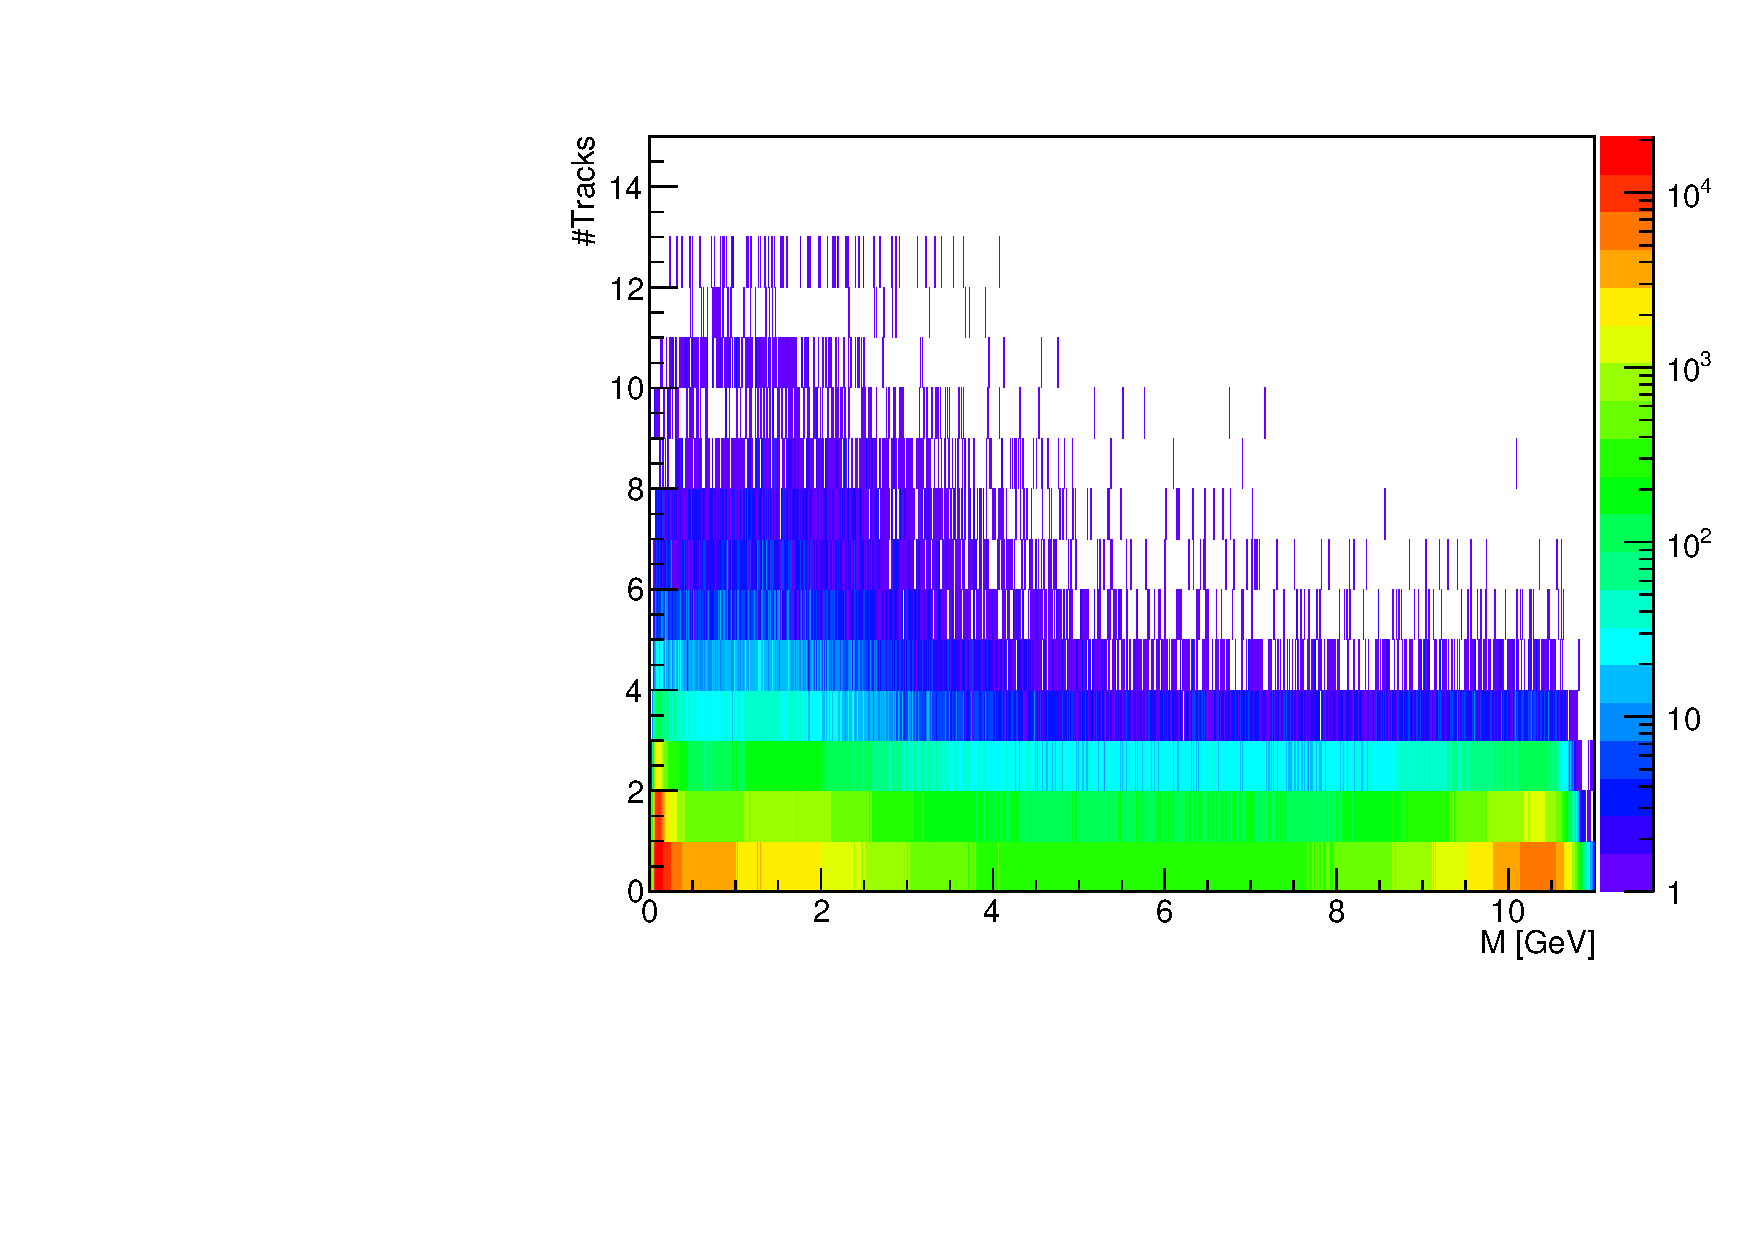
\includegraphics[width=8cm]{Plots/nTrM}
	\end{figure}
	
\end{frame}

\begin{frame}{The next Steps}
	\begin{itemize}
		\item Make more precise cuts
		\item Cut away the photons (middle peak)
		\item Make it run with MC files. (I already run on MC11 $\textrm{ee} \rightarrow \textrm{ee}$ with $10^7$ events but only 24 vpho survived the cuts)
	\end{itemize}
\end{frame}


\end{document}
